%************************************************
\chapter{Characterizing the evolution of genes and domains in mammals using \sw selective pressures}
%************************************************
\section{Introduction}

This chapter describes the use of \sw data to identify trends in the
evolution of protein-coding genes and domains, focusing on the
detection of \acp{psg}. I will first develop a number of methods for
using \sw estimates to identify signals of positive selection within
genes and domains and apply these methods to the \sw data generated in
Chapter \ref{ch_mammals1}. Next, to provide a higher-level
interpretation of these results I will use functional gene annotations
to identify categories enriched for genes with evidence of positive
selection in different species groups. Lastly, I will place these
results within the context of the literature by cirectly comparing the
sets of \acp{psg} identified by this and previously-published studies.

Since the first non-human mammalian genomes were sequenced, there has
been great interest in using comparative data to identify genes
showing signatures of positive selection in mammals. Much of this
interest stems from the prospect that such genes may reflect the
historical impact of natural selection acting to fix beneficial
mutations within a population over time---a major driving force in the
modern molecular interpretation of Darwin's theory of natural
selection \citep{Endo1996,Hughes1999}. Previous scans for positive
selection in primate genomes have revealed enrichments for \acp{psg}
related to sensory perception and olfaction \citep{Clark2003},
apoptosis and spermatogenesis \citep{Nielsen2005}, and iron ion
binding and keratin formation \citep{Macaque2007}; analyses in other
mammalian genomes have revealed largely similar patterns
\citep{Kosiol2008,Li2009a}. To explain the increased \dnds values
observed within \acp{psg}, three distinct evolutionary dynamics have
commonly been invoked: an evolutionary arms race between host and
parasite interacting genes \citep{Yang2005c}, sexual selection or
genetic conflict between the sexes \citep{Wyckoff2000,Clark2000}, and
functional adaptation following gene duplication \citep{Zhang2002}.

As the power of phylogenetic analysis using codon models depends
strongly on the amount of branch length encompassed by the species
being compared \citep{Anisimova2001,Anisimova2002}, there was some
reason to believe \emph{a priori} that the detection of \acp{psg}
using mammalian alignments incorporating \lcv genomes would be more
powerful than in previous whole-genome analyses, which typically
included 12 or fewer species across mammals and lower total branch
length \citep{ELLEGREN2008k}. However, differences in the specific
models used to detect positive selection are expected to affect the
sensitivities of one study compared to another \citep{Anisimova2009},
so the set of genes identified using the current methodology would
necessarily be expected to be a superset of those identified in
previous studies. Most large-scale studies have used the branch-site
test for positive selection \citep{Zhang2005}, while the results
described in this chapter were generated using \ac{slr}. I showed in
Chapter \ref{ch_indels1} that \ac{slr} has similar power to the
site-based test implemented in PAML for detecting \sw positive
selection, but no analysis has yet compared the differences in
\acp{psg} identified by site-specific and branch-site methods on a
large scale. For this reason, I hoped that a quantitative comparison
between \acp{psg} identified using the current methodology and those
found in previously-published studies may improve our understanding of
how similar or different the \acp{psg} identified by different methods
can be.

\section{Combining \sw estimates to identify positive selection}

In Chapter \ref{ch_mammals2} I covered the generation and analysis of
several highly filtered sets of genome-wide \sw selective pressures
within different groups of mammalian species. These \sw estimates were
used to characterize the global distribution of evolutionary
constraint and to compare overall levels of purifying and positive
selection between groups of mammalian species. The focus on individual
codons as an evolutionary unit of investigation is relatively
uncommon, but it allowed for large-scale differences in evolutionary
trends between species groups to be identified and for the impact of
different filtering schemes on overall signals of positive selection
to be easily evaluated.

The more traditional approach in comparative genomics has been to
model the protein-coding gene, as opposed the protein-coding amino
acid site, as the unit of analysis. For detecting positive selection,
the grouping of alignment sites into genes---which results in
identification of \acp{psg} instead of \acp{psc}---has three main
advantages. First, the combined analysis of many alignment sites
improves the accuracy of estimated evolutionary parameters and boosts
the power \ac{lr}-based tests for detecting positive selection. This
can be easily seen in the simulations of Anisimova and Yang
\citeyearpar{Anisimova2001,Anisimova2001}, which showed large power
differences for detecting positive selection in alignments simulated
with 100, 200, and 500 codons. Second, detailed studies of \sw
selective pressures in genes with strong signals of positive selection
have usually observed clusters of positively-selected sites
\citep{Sawyer2005a,Kosiol2008}, suggesting that the evolutionary
dynamics creating detectable signals of positive selection tend to
affect many functionally or structurally related amino acid sites
within a gene as opposed to a single site. These studies represent
empirical evidence that combining \sw estimates within genes is
biologically sensible. The third argument in support a gene-centric
analysis of positive selection is that in the absence of complete
protein structure information, much more tends to be known about
entire genes (through the results of high-throughput studies and
experiments in model organisms) than is known about individual
protein-coding sites. Thus, a gene-centric analysis allows a dataset
to be more easily analyzed in connection with abundant external
functional data, benefitting the biological interpretation of results.

A major issue in combining \sw estimates to identify \acp{psg} is that
of correcting for performing multiple \sw tests per gene. The \ac{slr}
method performs an independent statistical test at each site,
producing a sitewise statistic which can be compared to a \chisq
distribution to yield a p-value representing the strength of evidence
against strict neutral evolution \citep{Massingham2005}. When
combining these p-values to decide whether a gene contains significant
evidence for positive seletcion, one must take into account the number
of tests performed. For example, a 100-codon gene evolving under the
null model ($\omega=1$) would be expected to produce 5 sites with
p-values at a nominal \ac{fpr} of 0.05; correspondingly, the chance
that at least one site within the gene would have $p<0.05$ is
99.4\%. This is calculated as the complement of the probability that
no sites out of $n$ have $p<x$, which is $(1-x)^{n}$. Thus, if the set
of genes containing at least one site with nominal $p<0.05$ were
called \acp{psg}, nearly all genes evolving under the true null model
would be selected. In contrast, the \ac{lrt}s for positive selection
implemented in PAML only perform one statistical test per gene and do
not suffer from the same multiple testing problem. Clearly, some
procedure for correcting or combining the results from multiple tests
must be applied in order to identify \acp{psg} using \sw data in a
statistically controlled manner.

I tested 3 types of methods which are capable of correcting for
multiple \sw tests within genes to identify \acp{psg}: first,
adjusting significance thresholds to control the \ac{fwer}; second,
combining p-values from multiple tests to produce a single p-value
summarizing the overall evidence against the null hypothesis; third,
estimating empirical gene-wise p-values based on the genome-wide
distribution of \sw estimates. Each approach makes different use of
the \sw data from each gene to identify a set of significant \acp{psg}
and thus had the potential to yield a unique set of \acp{psg}. The
remainder of this section provides some background on each approach
and describes how it was applied to the current problem.

\subsection{Controlling the \ac{fwer}}

The \ac{fwer} is defined as the probability, for a given set of tests
performed, of one or more tests producing a false positive result. In
the example of a 100-codon gene evolving under the null model, the
\ac{fwer} at a nominal p-value of 0.05 was 0.994. Assuming an
appropriate uniform null distribution of p-values and independence
between tests, the \v{S}id\`{a}k equation (to which the more popular
Bonferroni correction is an easily computed approximation) identifies
the p-value threshold $x$ which is necessary to control the \ac{fwer}
at the desired level $\alpha$. The \ac{fwer} expected for a family of
$n$ tests thresholded at a nominal p-value of $x$ is $\alpha=1 - (1 -
x)^{n}$, so the p-value threshold necessary to control for a desired
\ac{fwer} can be found by rearranging the equation: $x=1 - (1 -
\alpha)^{1/n}$. A similar but more powerful approach to controlling
the \ac{fwer} is the step-up method from Hochberg; this method is
implemented internally by \ac{slr} for reporting the number of
positively- and negatively-selected sites after multiple testing
correction \citep{Hochberg1988,Massingham2005}.

I used the $p.adjust$ method from the R statistical project to apply
the Hochberg procedure to the set of \sw p-values from each gene; this
produced a new set of p-values representing the \ac{fwer} expected if
all sites with p-values equally or more extreme than the given site
were called significant. The overall p-value for each gene was taken
as the minimum \ac{fwer}-adjusted p-value across all sites.

One weakness of this approach is that the evidence for assigning
positive selection comes only from the site with the most extreme
\slrt, ignoring any signal of positive selection from sites with
weaker p-values. As it has been previously observed that \acp{psg}
often contain multiple sites subject to similar elevated dN/dS levels
\citep{Sawyer2005a,Kosiol2008}, the gene-wise p-values resulting from
the above approach to controlling the \ac{fwer} may lack power to
detect positive selection in genes with many sites showing moderate to
strong evidence for positive selection. The next two methods described
are both sensitive to more than just the most significant site, making
them potentially more powerful for identifying \ac{psg} in a
statistically-controlled manner.

\subsection{Combining p-values}

The second approach to multiple testing directly addresses this
problem by combining p-values from a series of independent tests,
producing an overall p-value for the null hypothesis given the set of
tests performed. The motivation behind such methods is that moderately
significant results from independent tests of a common null hypothesis
should be considered as good or better evidence than one strongly
significant test. Many different specific techniques of this type have
been discussed in the literature (see \citet{Cousins2007} for an
extensive annotated bibliography). Two of the most popular methods are
Fisher's combined probability test and Stouffer's method
(\citealp{Fisher1932}; \citealp{Stouffer1949}; reviewed in
\citealp{Whitlock2005}). Briefly, each method combines p-values from
independent tests in some way (Fisher's test takes the product of all
p-values, while Stouffer's method transforms p-values into normal
quantiles and sums the resulting z-scores) and compares the resulting
statistic to the expected distribution given a null distribution of
the same number of input p-values. Comparisons of both tests suggested
that they provide similar power overall, but Stouffer's method
generally yields smaller p-values when the input p-values are more
similar and Fisher's test yields smaller p-values when the input
p-values vary widely \citep{Darlington2000}. When the distribution of
input p-values is nonuniform or the number of tests is large, however,
performance can be reduced. It has been noted that a relatively small
number of large p-values can limit the power of Fisher's test
\citep{Zaykin2002}, and the Stouffer method should be equally
sensitive to small and large p-values. Since the majority of mammalian
protein-coding sites showed moderately strong signals of purifying
selection in the global distribution, the distribution of one-sided
p-values for positive selection would be heavily weighted towards 1
for the set of \sw estimates in most genes. As a result, both the
Fisher and Stouffer methods were expected to lack power to identify
\acp{psg}, as the dominant signal of purifying selection in most genes
would tend to produce non-significant combined p-values for positive
selection even when strong evidence for positive selection exists.

The variants of Fisher's and Stouffer's methods which incorporate a
truncation step (i.e., including only p-values below a pre-specified
threshold to calculate the combined statistic) provided a potentially
more powerful approach to combining \sw p-values within genes
\citep{Darlington2000,Zaykin2002,Zaykin2007}. Zaykin et
al. \citeyearpar{Zaykin2002,Zaykin2007} showed that the \ac{tpm}, a
truncated version of Fisher's product method, is well-suited for
large-scale genomics experiments where the number of tests is large
and the standard methods lack power. The authors suggest a truncation
threshold of $p<0.05$ provides a good balance of sensitivity and
power, and they note that the method is asymptotically equivalent to
Fisher's combined test as the p-value trunctation is increased to
1. Thus, the truncation threshold determines the extent to which the
method focuses on more significant test results. The test statistic is
calculated as the product of all p-values below the truncation
threshold, and in the implementation provided by Zaykin get
al. \citeyearpar{Zaykin2002} the significance of the statistic is
determined by simulation based on the null model. As an example, for a
gene with 100 sites and 5 where $p<0.05$, the test statistic would be
the product of those 5 p-values and its significance would be tested
by generating 5,000 replicates under the null model (i.e., uniformly
distributed p-values) using the same $p<0.05$ criterion to calculate
the truncated product of p-values.

To explore the behavior of the \ac{tpm} at various p-value truncation
thresholds, I used the implementation provided by Zaykin et
al. \citeyearpar{Zaykin2002} to calculate combined p-values at
truncation thresholds corresponding to a nominal 5\%, 10\%, 20\%, and
50\% \sw \acp{fpr}. I also calculated a combined p-value using
Fisher's standard combined method to test the hypothesis that the
method lacked power to detect \acp{psg} in protein-coding genes due to
the presence of many purifying sites.

\subsection{Assigning empirical p-values based on the global \sw distribution}

The previous two approaches are fairly generic statistical methods,
with formulas whose accuracy depends on the assumption of
uniformly-distributed p-values under the null hypothesis. Since the
overall distribution of one-tailed p-values from \sw estimates is far
from uniform, however, the large proportion of sites with strong
evidence for purifying selection may cause problems when a uniform
distribution of p-values is assumed. This problem is alleviated
somewhat by the fact that \ac{fwer} control mainly uses only the most
significant test result to identify a \acp{psg}. The sensitivity of
the \ac{tpm} method to largely non-uniform p-values should also be
reduced, as sites with p-values above a certain threshold from the
calculation of the combined statistic, thus avoiding undue influence
from non-significant p-values. Still, the apparent mismatch between
the neutral null model tested by \ac{slr} and the large majority of
sites evolving under purifying selection suggested that tests based on
the theoretical distribution of \ac{lrt} statistics may be overly
conservative. For the confident identification of \acp{psg} this may
be desirable, but for the global analysis of functional trends in
genes subject to \acp{psg}, a less conservative approach should
provide more signal. Given the large set of \sw estimates available
for each species group, the identification of \acp{psg} based on
empirical p-values was an attractive alternative approach, with
potentially more power to detect genes with significant deviations
from the observed genome-wide distribution of \slrt statistics within
each species group \citep{Noble2009a}.

I implemented a randomization method to assign an empirical p-value to
each gene based on the length of the gene and the number of sites with
p-values below a certain pre-specified significance threshold. This
design shares some characteristics with the \ac{tpm} method, as the
test statistic comes from the subset of sites exceeding a certain
significance threshold. The test statistic here, however, was a simple
count of the significant sites. To assess the significance of the
observed count for a given gene, a set of pseudo-replicate genes (each
with the same number of sites as the real gene) was generated by
sampling with replacement from the genome-wide set of \sw
estimates. Using the pre-specified significance threshold, the number
of significant sites from each replicate was counted. Given $n$, the
number of replicates, and $r$, the number of replicates with as many
or more significant sites than the observed count, the empirical
p-value was calculated as $(r+1) / (n+1)$ \citep{North2002}. This
method was applied to each gene using 100,00 replicates; as with the
\ac{tpm} method, the effect of different truncation thresholds was
assessed by separately calculating empirical p-values using nominal
0.05\%, 1\%, 5\%, and 10\% \ac{fpr} thresholds.


\section{Analysis of \acp{psg} identified using \sw selective pressures}

The methods described above was applied to \sw estimates from each of
the 10 species groups 3 levels of \sw filtering from Chapter
\ref{ch_mammals1}.

To assess the overall behavior of each method, I first looked at the
distribution of p-values for different species sets using the
conservatively-filtered \sw data. Figure \ref{fig_psg_pvals} shows the
distribution of gene-wise p-values for 10 species groups using the
Hochberg, Fisher, \ac{tpm}, and empirical methods described
above. (Note that for the \ac{tpm} and empirical methods, only one
truncation threshold is shown for simplicity; the distributions of
p-values for the other truncation thresholds were qualitatively
similar.) As expected, Fisher's product method produced very few
p-values below 1, showing little to no power to detect positive
selection in any species group. The \ac{tpm} was slightly more
sensitive than Fisher's product method with roughtly 10\% of genes
yielding p-values below 1 for the Mammals species group; the
comparison between Fisher's method and the \ac{tpm} showed that the
truncation slightly increased the sensitivity of the method, but the
overall sensitivity remained low with very few genes producing low
p-values.

\begin{figure}
\centering
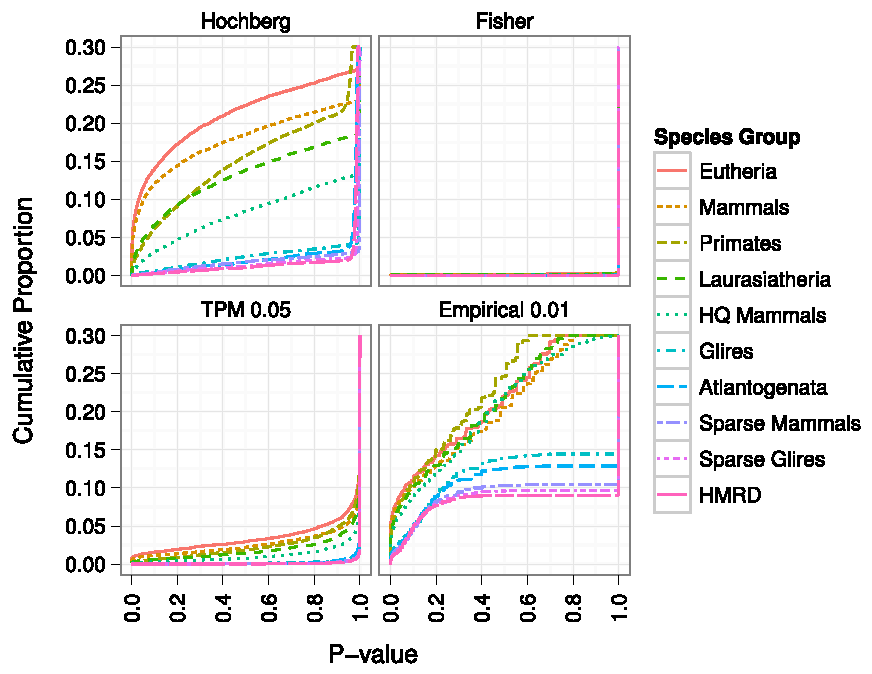
\includegraphics[scale=0.9]{Figs/psg_pvals.pdf}
\caption{Cumulative distributions of gene-wise p-values for positive
  selection resulting from 4 different methods for combining \sw
  estimates within genes. Note that the species groups are listed in
  order of their cumulative proportions at a p-value of 0.5 for the
  Hochberg method. To more clearly show the separation between species
  groups at lower y-values, cumulative proportions above 0.3 are not
  shown.}
\label{fig_psg_pvals}
\end{figure}

The Hochberg and empirical methods both showed much greater
sensitivity and revealed strong differences in the distributions of
p-values between species groups. For the Hochberg method, Eutheria and
Mammals groups showed a large proportion of p-values in the realm of
significance, with roughly 10\% of genes having $p<0.05$. Primates and
Laurasiatheria clustered together with the next highest proportion of
low p-values (roughly 5\% with $p<0.05$), followed by the HQ Mammals
group with roughtly 2\% of genes with $p<0.05$. The other species
groups all showed no visible enrichment for low p-values, with a
largely uniform distribution of p-values in the range of $0<p<1$ and
less than 5\% of genes with a p-value below 1. The empirical method
produced two tight clusters of species groups: the first cluster, with
roughly 5-7\% of genes with $p<0.05$, contained Eutheria, Mammals,
Primates, Laurasiatheria and HQ Mammals; the second cluster, with
roughly 2\% of genes having $p<0.05$, contained the other 5 species
groups. Note that the cumulative curve for species groups in the lower
cluster levels off at around $p=0.2$. This leveling off occurred at
the maximum p-value given to genes with at least one site below the
truncation threshold; the substantial fraction of genes with zero
sites below the truncation threshold yielded p-values near to 1.

The major differences between the Hochberg and empirical methods were
the tighter clustering of the empirical p-values for the 5 species
groups with greater evidence for positive selection and the greater
proportion of low empirical p-values for the 5 species groups with
less evidence for positive selection. Both differences could be
explained by the fact that the Hochberg method assessed significance
based on the absolute magnitude of the \ac{lrt} statistic for positive
selection, while the empirical method assessed significance based on
the magnitude of evidence for positive selection \emph{relative} to
all \sw estimates for a given species group. This had the effect of
increasing the proportion of genes with low p-values for species sets
with less branch length (e.g., Primates, Laurasiatheria, and HQ
Mammals) or less overall evidence for positive selection (e.g., the
five species groups from the lower cluster). As a result, although the
overall pattern for each method was somewhat similar, it appeared that
the empirical method provided greater sensitivity to detect signals of
positive selection while accounting for differences in branch lengths
and the background distribution of \sw selective pressures.

In order to identify a set of confident \acp{psg} for each method it
was important to control for multiple testing across genes, since
several thousand genes were independently tested for positive
selection. This multiple testing issue, resulting from performing many
tests across a genome, was distinct from the previously discussed
issue of multiple testing across \emph{sites} within a gene. In the
case of testing many sites within a gene, the driving question was an
overall hypothesis about the gene (e.g., does the gene contain any
positively-selected sites or not) and the appropriate error rate to
control was the \ac{fwer}. In contrast, the goal of testing many genes
across a genome was not to answer a specific global question (e.g.,
are \emph{any} genes under positive selection), but rather to identify
candidates with a reasonably low number or proportion of likely false
positive results. For this purpose, the \ac{fdr}, defined as the
expected proportion of rejections of the null hypothesis that are
false, is a powerful and easily interpreted type of statistical
control \citep{Benjamini1995}. Thus, the \acp{psg} reported in Table
\ref{table_psg_summary} are those genes which remained significant
after controlling for an expected FDR$<0.1$ using the Benjamini
Hochberg method \citep{Benjamini1995}.

\bbtable
\centering \scriptsize
\begin{tabular}{llrrrrrrrrrrrrr}
\toprule
Filter & Species Group & Genes & \wa & \wg & \psghoch & \psgfisher & \psgtfifty & \psgttwenty & 
\psgtten & \psgtfive & \psgeohfive & \psgeone & \psgefive & \psgeten \\
  \midrule

\input{Tables/psg_summary_default.txt}

  \midrule

\input{Tables/psg_summary_stringent.txt}

  \midrule

\input{Tables/psg_summary_pfam.txt}

\bottomrule
\end{tabular}
\caption{\acp{psg} identified using \sw data with 3 \sw filters, 10
  species groups and different methods to combine p-values across
  sites. The columns \wa and \wg present the arithmetic and geometric
  means, respectively, of the gene-wide \omg values estimated by
  \ac{slr}. To identify \acp{psg}, only genes with at least 50 \sw
  estimates from the given species group and filter were tested. The
  Benjamini-Hochberg method was used to identify \acp{psg} significant
  at FDR$<0.1$ for all methods. Hoch.---Hochberg's method for
  \ac{fwer} control; Fis.---Fisher's combined p-value test;
  TPM---truncated product method using 50\%, 20\%, 10\% and 5\%
  \ac{fpr} thresholds; E---empirical p-values using 0.5\%, 1\%, 5\%
  and 10\% \ac{fpr} thresholds.}
\label{table_psg_summary}
\eetable

Table \ref{table_psg_summary} provides a summary of \acp{psg}
identified by each method for each \sw filter and species group. Only
genes with at least 50 \sw estimates were tested, resulting in
different numbers of genes for different species groups and \sw
filters. Groups containing fewer species, such as Atlantogenata and
HMRD, tended to contain slightly fewer genes than larger groups; this
mirrored differences between species groups in the genome-wide number
of \sw estimates seen in Chapter \ref{ch_mammals1} (see Table
\ref{table_pset_summaries_1}).

The pattern of \ac{psg} counts was qualitatively similar between
different \sw filters, with fewer \acp{psg} found using more stringent
filters. For each combination of species group and method, the
greatest number of \acp{psg} was generally found using the relaxed
filter, fewer were found using the conservative filter, and the fewest
were found using only sites within Pfam domains. This was partially
due to the lower total number of genes retained for analysis with the
two more conservative filters: for the Mammals species group, 15,946
genes contained at least 50 sites for analysis using the default
filter, while the conservative and Pfam filters resulted in only
10,192 and 10,587 genes, respectively. Even after accounting for the
different total gene counts in different filters, the number of
\acp{psg} as a proportion of all genes was still reduced in the more
conservative filters: as an example, for \acp{psg} identified in the
Mammals group using Hochberg \ac{fwer}, 7.8\% of genes were \acp{psg}
using the relaxed filter, 4.7\% using the conservative filter, and
2.8\% using only sites within annotated Pfam domains. A similar trend
was observed for the other \acp{psg} identification methods, showing
that the conservative and Pfam filtered datasets contained
progressively lower proportions of genes subject to positive
selection. This corresponded well with the pattern seen in Chapter
\ref{ch_mammals1} for the prevalence of positively-selected sites.

Comparing between the different methods for identifying \acp{psg}, the
Hochberg \ac{fwer} control and empirical p-value methods were much
more sensitive than the Fisher and \ac{tpm} methods, as expected from
the p-value distributions in Figure \ref{fig_psg_pvals}. The Fisher
method was the most conservative, identifying a vanishingly small
number of \acp{psg} in all species groups. Comparing results from the
\ac{tpm} method at different truncation thresholds, the method provded
to be increasingly more sensitive as the truncation threshold was
decreased; in the Mammals group using the conservative filter, 55
\acp{psg} were identified with a truncation threshold of $p<0.05$. The
empirical method was the least sensitive with a truncation threshold
of $p<0.01$, with increased sensitivity using the lowest threshold
($p<0.005$) and the two higher thresholds ($p<0.05$ and $p<0.1$). The
Hochberg method and the most conservative empirical method yielded 474
and 585 \acp{psg} in the Mammals group, respectively.

Although the Hochberg and empirical methods resulted in similar
numbers of \acp{psg} for the Mammals species group, the empirical
method identified the greater number of \acp{psg} in the smaller
species groups. The pattern of Hochberg \ac{psg} counts across species
groups was reminiscent of the pattern of significant \acp{psc}
identified after controlling the \ac{fdr} (Table
\ref{table_pset_summaries_2}): Mammals and Eutheria yielded several
hundred \acp{psc} and \acp{psg}, Primate and Laurasiatheria yielded a
much smaller but still non-zero number, and the other species groups
yielded none. The consistency of this pattern between \acp{psc} and
\acp{psg} reflected the fact that the Hochberg method for identifying
\acp{psg} was sensitive largely to the existence of any one site
within a gene having a very strong signal of positive selection. Thus,
only the species groups with a large total branch length and a high
prevalence of positive selection produced a large number of Hochberg
\acp{psg}.

In contrast, \acp{psg} from empirical p-values reflected a significant
clustering of less extreme \acp{psc}. As a result, the empirical
method identified some \acp{psg} in species groups where the Hochberg
method identified none. The qualitative pattern between species groups
was largely similar to that seen for the Hochberg \acp{psg}: using the
conservative filter and the empirical method with a truncation
threshold of $p<0.01$, Mammals and Eutheria yielded around 600
\acp{psg}, Primates, Laurasiatheria and HQ Mammals produced around
400, and most other species groups had 50 or fewer \acp{psg}. The
species group with the most striking difference between the Hochbeg
\acp{psg} and the empirical \acp{psg} was the HQ Mammals group, which
had zero Hochberg \acp{psg} but several hundred empirical
\acp{psg}. This was consistent with the intermediate location of the
cumulative curve for HQ Mammals under the Hochberg method in Figure
\ref{fig_psg_pvals}; although this species group showed a greater
enrichment of low p-values than the lowest cluster of curves, it was
not strong enough to produce any significant genes at FDR$<0.1$.

In summary, the 3 types of methods for combining \sw estimates to
identify \acp{psg} showed very different performance patterns across
the different species groups. While the \ac{tpm} and Fisher's method
have been extensively used in large-scale studies, they appeared to
lack power in this application. Control of the \ac{fwer} or the use of
empirical p-values yielded greater numbers of \acp{psg}. Using these
methods to identify \acp{psg}, the 10 species groups fell into 2
clusters, each with a very different proportion of identified
\acp{psg}.

\subsection{Overlaps between positively-selected genes in different species groups}

\begin{figure}
\centering
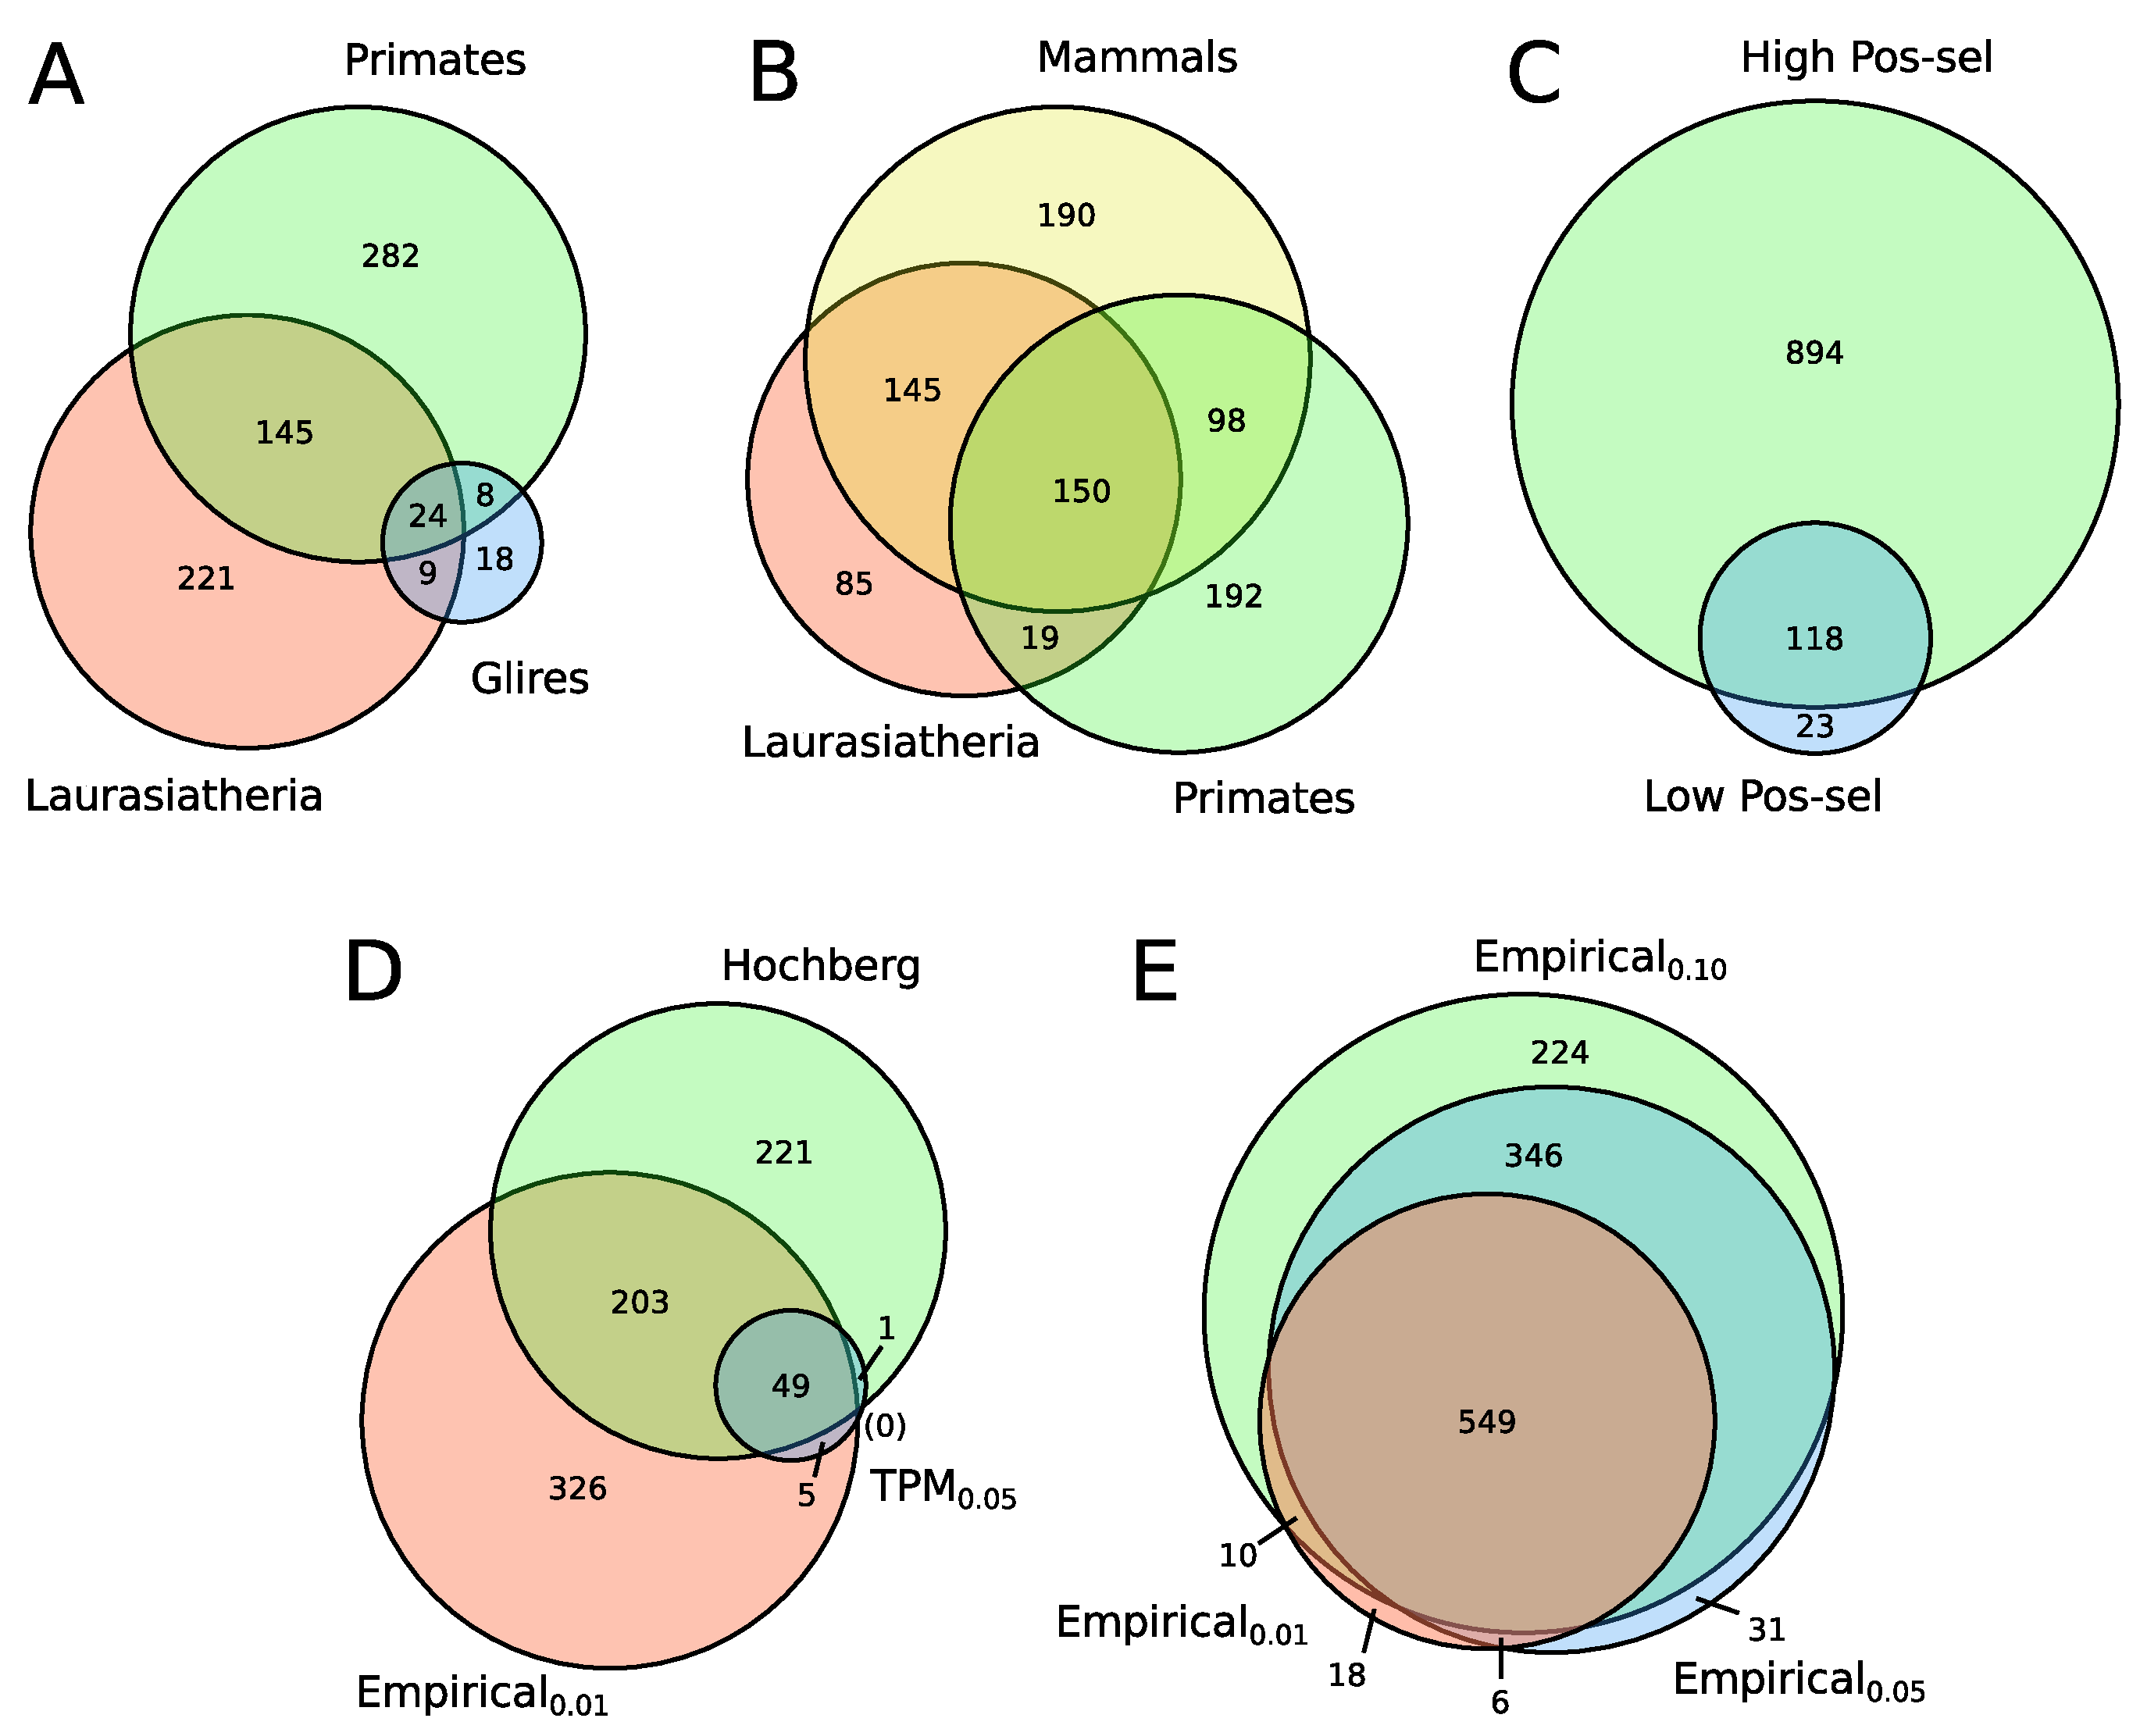
\includegraphics[scale=0.3]{Figs/psg_venns.pdf}
\caption{Venn diagrams of \acp{psg} identified in different species
  groups and using different methods. (A) \acp{psg} identified using
  empirical p-values in Primates, Glires, and Laurasiatheria. (B)
  \acp{psg} identified using empirical p-values in
  Mammals. Laurasiatheria and Primates. (C) \acp{psg} identified using
  empirical p-values in species groups with high and low levels of
  positive selection. (D) \acp{psg} identified in the Mammals group
  using three different methods for combining \sw estimates within
  genes. (E) \acp{psg} identified in the Mammals group using the
  empirical p-value method with 3 different truncation thresholds:
  $p<0.01$ (smallest circle, left), $p<0.05$ (middle circle, right),
  $p<0.10$ (largest circle, top).}
\label{fig_psg_venns}
\end{figure}

Using the sets of significant \acp{psg} from Table
\ref{table_psg_summary}, it was possible to identify how many
\acp{psg} were shared between, or unique to, different species groups
or methods. Unless otherwise specified, all future analyses in this
chapter will be derived from the conservatively-filtered dataset.

I first looked at the distribution of \acp{psg} from the empirical
method with a $p<0.01$ truncation threshold across species
groups. Overall, a total of 1035 out of 11520 genes, or 8.9\% of those
investiated, were identified as a \ac{psg} in at least one of the
species groups. Figure \ref{fig_psg_venns} shows a more detailed
breakdown of how many \acp{psg} were shared between various species
groups. Figure \ref{fig_psg_venns}A compares genes from the three
major mammalian superorders, showing that Primates and Laurasiatheria
share roughly a third of their \acp{psg} and that around two-thirds of
\acp{psg} in Glires are also significant in Primates, Glires, or
both. Figure \ref{fig_psg_venns}B looked at \acp{psg} shared between
Primates, Laurasiatheria, and Mammals (which contained all of the
species within the Primates and Laurasiatheria groups), showing
roughly equal mixtures of shared and unique genes. Finally, I split
the 10 species groups into 2 clusters based on the prevalence of
\acp{psg}: Mammals, HQ Mammals, Eutheria, Primates and Eutheria were
considered ``High Pos-sel'' groups, and the rest were considered ``Low
Pos-sel'' groups. Figure \ref{fig_psg_venns}C shows the overlap
between the union of \acp{psg} identified in each group; \acp{psg}
from the High Pos-sel cluster of species groups is largely a superset
of those from the Low Pos-sel cluster, with only 23 \acp{psg} unique
to the species groups which showed less overall positive selection.

Expanding the count to include \acp{psg} identified by the Hochberg,
Fisher, and truncated product methods (at a truncation threshold of
$p<0.05$), the total number of \acp{psg} identified was 1300, or
11.3\% of all genes tested. Compared to the 1035 from the empirical
method alone, the additional 265 genes came from the Hochberg method
in the Eutheria and Mammals groups. Figure \ref{fig_psg_venns}D shows
the overlap of \acp{psg} identified in the Mammals group by different
methods; while the \ac{tpm} yielded no unique \acp{psg}, a large
number of the Hochberg genes were unique, indicating that the Hochberg
and empirical p-value methods were sensitive to different patterns of
positively-selected sites within genes. In contrast, Figure
\ref{fig_psg_venns}E shows that the different variants of the
empirical method using different truncation thresholds yielded largely
the same set of \acp{psg}, but with increasing sensitivity as the
truncation threshold was relaxed from $p<0.01$ to $p<0.10$.

\section{Functional analysis of \acp{psg} and comparison to previous studies}

I used \ac{go} term annotations from the \ens database to identify
functional categories enriched for \acp{psg}. \ac{go} annotations for
all human genes were downloaded from version 64 of \ens and were
applied to the mammalian alignment containing each human gene. As the
\ac{go} ontology contains links between terms forming a directed
acyclic graph, I followed the common practice of applying the set of
all ancestral, and thus less-specific, terms to each gene as well
\citep{Rivals2007}. Only terms within the Biological Process ontology
were included in this analysis, as the Molecular Function and Cellular
Component hierarchies contain less information on the types of
processes generally associated with the presence of positive selection
in mammalian genes \citep{Macaque2007}.

Two methods were employed to identify \ac{go} terms enriched for
\acp{psg}. First, a simple test for independent association was
performed for each term: a 2x2 contingency table was filled with the
counts of \acp{psg} and non-\acp{psg} which were annotated and not
annotated with the current term (each combination of which filled one
cell of the table), and \ac{fet} was used to perform a one-sided test
for independence of rows and columns. A highly significant \ac{fet}
p-value thus represented strong evidence for a positive association
between a gene being positively-selected and being annotated with the
given term \citep{Rivals2007}. To control for multiple tests being
performed, I excluded all terms containing fewer than 5 \acp{psg} (to
reduce the number of tests performed and to avoid including highly
specific and less biologically-informative \ac{go} terms) and used the
Benjamini-Hochberg method to identify the \ac{fet} p-value needed to
control for an expected \ac{fdr}$<0.1$ within each set of
\acp{psg}. The second method I used to assess significance was the
\texttt{weight} algorithm from the \topgo program
\citep{Alexa2006a}. The \texttt{weight} algorithm also uses \ac{fet}
to identify significant associations between terms and genes of
interest, but it accounts for the fact that gene annotations for
nearby terms in the \ac{go} graph structure are highly correlated by
reducing the significance of terms which have more specific,
significantly-enriched descendant terms. The result of this weighting
is that clusters of closely-related and highly significant terms,
which may otherwise clutter the list of top \ac{fet} results with an
uninformative set of very similar terms, are thinned out by reducing
the p-values of the less-specific ancestors. Only terms which were
significant by both \ac{fet} (FDR$<0.1$) and the \texttt{weight}
algorithm ($p<0.1$) were included in the top and bottom sections of
Table \ref{table_go}. Terms with more than 300 or fewer than 30
annotated genes were also excluded from inclusion in the top or bottom
sections of Table \ref{table_go} for clarity.

These two methods were applied to several sets of \acp{psg} in order
to assess the consistency of enriched terms between different methods
for identifying \acp{psg} and different species groups. The
conservatively-filtered dataset was used for all tests. Each set of
enriched terms was assigned a letter for identification in Table
\ref{table_go}; those letters are included here in parentheses for
reference. From the Mammals group, I tested for enriched \ac{go} terms
in the 474 \psghoch \acp{psg} (\texttt{H}), the 585 \psgeone \acp{psg}
(\texttt{M}), the 934 \psgefive \acp{psg} (\texttt{m}), and the 202
genes in the top 2\% genome-wide by overall \dnds value
(\texttt{D}). The latter group was defined using gene-wide \dnds
values output by \ac{slr}, based on fitting a M0-like codon model to
the mammalian alignment. To evaluate \acp{psg} identified in the
mammalian superorders, I tested the 459 \psgeone \acp{psg} from
Primates (\texttt{P}), the 409 \psgefive \acp{psg} from Glires
(\texttt{g}), and the 400 \psgeone \acp{psg} from Laurasiatheria
(\texttt{L}). Finally, the set of 273 genes with independent evidence
for positive selection in each of the Primates, Glires, and
Laurasiatheria groups was obtained by taking the least significant
\psgefive p-value for each gene from each species group and
identifying genes which remained significant (\texttt{i}). Note that
groups indicated by lowercase letters correspond to those using the
less conservative \psgefive \ac{psg} definition.

In order to facilitate a comparison with functional associations
reported in previously-published studies, I also collected the lists
of terms enriched for \acp{psg} from Clark et
al. \citeyearpar{Clark2003} (\texttt{C}), the Rhesus Macaque Genome
Sequencing and Analysis Consortium \citeyearpar{Macaque2007}
(\texttt{R}), and Kosiol et al. \citeyearpar{Kosiol2008} (\texttt{K}).

\bbtable
\centering \scriptsize
\begin{tabular}{llllrrrrrl}
\toprule

\multicolumn{2}{c}{\ac{go} Term} & \multicolumn{2}{c}{Enriched in} & \multicolumn{6}{c}{Values for Mammals \psgefive (label \texttt{M} in ``This Study'' column)} \\

\cmidrule(r){1-2}
\cmidrule(r){3-4}
\cmidrule(r){5-10}

ID & Description & \multicolumn{1}{c}{This Study} & \multicolumn{1}{c}{Lit.} & \ac{fet} & \topgo & Ann.  & Sig. & Exp. & Top 5 Genes \\

\midrule
\multicolumn{4}{l}{Top 10 Enriched Terms} & & & & & & \\
\midrule

\input{Tables/psg_go_top.txt}

\midrule
\multicolumn{4}{l}{Other Terms Commonly Identified in the Literature} & & & & & & \\
\midrule

\input{Tables/psg_go_them.txt}

\midrule
\multicolumn{4}{l}{Other Terms Identified in This Study but Not in
  the Literature} & & & & & & \\ \midrule

\input{Tables/psg_go_me.txt}


\bottomrule
\end{tabular}
\caption{Example \ac{go} terms enriched for \acp{psg} in this study
  and in the literature. Top section: the 10 terms most significantly
  enriched for \psgefive \acp{psg} in the Mammals species
  group. Middle section: other terms found in at least 2 of 3
  published genome-wide scans. Bottom section: other terms enriched
  for \acp{psg} in this study but not in the literature. The presence
  or absence of characters under the columns ``This Study'' and
  ``Lit.'' indicates which sets of genes from this or
  previously-published studies showed enrichment for \acp{psg} for
  that term (see text for definitions). The last 6 columns show values
  from the Mammals \psgefive set, corresponding to the `\texttt{M}'
  flag; bold P-values indicate significance (FDR$<0.1$ for \ac{fet}
  and p$<0.05$ for \topgo). Genes discussed in the text are presented
  in bold face. Lit.---literature; \ac{fet}---Fisher's Exact Test;
  Sig.---Significant; Exp.---Expected.}
\label{table_go}
\eetable

Table \ref{table_go} summarizes the results of the \ac{go} term
enrichment tests, showing for three sets of terms which groups of
genes from this study, and which previously-published studies,
identified a significant enrichment of \acp{psg}.

The top section shows 10 of the \ac{go} terms most strongly enriched
for Mammalian \psgefive \acp{psg} according to \ac{fet}. The top few
terms, including \emph{inflammatory response}, \emph{innate immune
  response}, \emph{defense response to virus} and \emph{defense
  response to bacterium}, represented genes involved in host defense
and immune response---two of the functions most commonly associated
with positive selection in mammals \citep{Nielsen2005b}. Accordingly,
the top four terms were identified in one or two previously-published
studies and in most or all of the species groups and \acp{psg}
identification methods evluated in this study. Interestingly, the term
\emph{mitotic prometaphase} was associated with \acp{psg} in almost
all gene sets from this study, but it was not found by any of the sets
of enriched terms from the literature. The next several terms, most of
which were not found in the literature, showed a more mixed pattern of
enrichment across gene sets from this study. Some of these terms,
including \emph{mitosis} and \emph{centrosome organization} were
connected to the more strongly-enriched \emph{mitotic prometaphase}
term and showed many of the same significant genes; others, such as
\emph{platelet degranulation} and \emph{leukocyte migration} were
distinct in function and composition of Mammalian \psgefive \acp{psg}.

The middle section of Table \ref{table_go} focuses on \ac{go} terms
commonly associated with \acp{psg} in the literature which were not
included in the 10 top terms, showing all terms identified in at least
2 of the 3 previously published studies. The first 5 terms largely
recapitulated those included in the top section relating to defense
response and inflammation, all of which were identified in most gene
sets from the current study. The next several terms, including
\emph{sensory perception of taste} and \emph{cell surface receptor
  linked signaling}, were more related to sensory perception and were
uniformly not associated with \acp{psg} in this study. The lack of an
association for these terms in the current study was surprising, as
olfaction and sensory perception have been among the most consistently
identified functional categories in large-scale scans for positive
selection \citep{Nielsen2005,Nielsen2005b}. One explanation for this
difference may be that the removal of highly-duplicated genes from the
conservatively-filtered dataset has reduced the number of olfactory
and sensory genes available for analysis. While there was some
evidence that the current dataset was depleted of olfactory genes
compared to previous analyses (according to Table \ref{table_go} only
17 genes were annotated with \emph{sensory perception of smell}, while
Kosiol et al. \citeyearpar{2008} analyzed 229 such genes), the number
of genes annotated with \emph{sensory perception} (274) and
\emph{sensory perception of chemical stimulus} (36) were still large
enough to produce a significant enrichment if one existed. Other
possible explanations included the possibility that
positively-selected sensory genes were more prone to exclusion from
the current analysis for other reasons (for example, if their
alignments contained more clustered \nsyn substitutions) or less
sensitivity in the current study to the patterns of positive selection
occurring in sensory perception genes.

The bottom section of Table \ref{table_go} shows the remainder of
terms which were identified in the current study, but not in previous
studies providing \ac{go} term enrichments, as associated with
\acp{psg}. The first term, \emph{double-stranded break repair}, was
identified in 3 of the 8 gene sets, with the association with
\acp{psg} driven by genes such as \gene{SETX}, a RNA helicase which
causes ataxia and lateral sclerosis when defective
\citep{Suraweera2007}, and \gene{BRCA2}, a tumor suppressor gene for
which a common allele is associated with an increased risk of breast
cancer and whose close relative, \gene{BRCA1}, has been shown to be
positively selected in mammals \citep{Huttley2000a}. Some of the next
terms, including \emph{cell division} and \emph{T cell costimulation}
and \emph{TNF superfamily cytokine production}, were similar to other
terms in the first two sections and contained similar sets of
\acp{psg}, but the terms \emph{organic anion transport} and
\emph{spermatogenesis} were quite distinct in their function and set
of associated \acp{psg}. The anion transport term contained largely
members of the \ac{slc} gene superfamily, a 300-strong group of
membrane-bound transporter genes \citep{He2009}, while the
\emph{spermatogenesis} category has been widely reported in other
studies of mammalian positive selection not included in Table
\ref{table_go}
\citep{Torgerson2002,Swanson2003,Clark2005,Nielsen2005}.

The \ac{go} term enrichments indicated a strong prevalence of positive
selection in genes related to core cellular processes such as cell
division and DNA repair. Many of these associations were noted and
discussed by Nielsen et al. \citeyearpar{Nielsen2005}, who
hypothesized an interesting connection between \acp{psg} and
cancer-related genes in these functional categories. Nielsen et al.
suggested that cancer-related genes, which are often involved in cell
proliferation and apoptosis pathways, may be likely targets of
positive selection resulting from genetic conflict due to their
involvement in processes known to lead to positive selection, such as
the proliferation of immune cells \citep{Sawyer2005a} or sperm
competition \citep{Torgerson2002,Clark2005}. This hypothesis was
developed and expanded by Crespi and Summers \citeyearpar{Crespi2006},
who analyzed the results of several scans for positively-selected
genes through the lens of cancer risk. Crespi and Summers argued that
positive selection resulting from ``antagonistic coevolution'' between
various entities (e.g., hosts and parasites, parents and offspring, or
sperm cells and eggs) has been the driving force behind the evolution
of increased cancer risk. Although similar trends were observed by
Nielsen et al., the current study provided additional support for an
association between positive selection and cancer-related genes,
expanding the list of \acp{psg} in functional categories related to
cancer progression and containing known tumor suppressor genes.

A more surprising result from the \ac{go} term analysis was the strong
enrichment of \acp{psg} in terms related to mitosis and chromosome
segregation. None of these terms were identified in the previous
studies analyzed, but I found strong enrichments for terms such as
\emph{mitosis}, \emph{centrosome organization}, and \emph{chromosome
  segregation}. All of these terms were identified as enriched for
\psgeone \acp{psg} in Mammals, while \emph{centrosome organization}
was enriched for \psgeone in Laurasiatheria and for \psgefive in
Glires. Among the top \acp{psg} within these terms were \gene{HAUS6},
a member of the HAUS microtubule-binding complex which is vital to the
mitotic spindle assembly and maintenance of the centrosome,
centrosomal proteins \gene{CEP152} and \gene{CEP250}, and several
centromere proteins including \gene{CENPT}, \gene{CENPI},
\gene{CENPQ}, and \gene{CENPH}. There has been great interest
surrounding the evolution of centromeric DNA and proteins ever since
Henikoff, Ahmad and Malik first proposed the ``centromere paradox''
\citeyearpar{Henikoff2001}. Based on the observation that both
centromeric DNA and centromere-related proteins were rapidly evolving
in animals, the authors proposed an ongoing genetic conflict between
centromeric DNA and proteins resulting from the unequal transmission
of chromosomes during female meiosis
\citep{Henikoff2001,Malik2002,Malik2009}. Initial comparative analysis
of the major centromeric protein \gene{CENPA} gene showed it to be
positively-selected in \emph{Drosophila} and \emph{Arabidopsis} but
not in mammals, while a more recent study in primates identified
positively-selected residues in \gene{CENPA} and three other
centromeric proteins \citep{Schueler2010}. This study provided
large-scale corroboration of the result from primates, showing that
positive selection in centrosomal and centromeric proteins is a major
component of the overall set of \acp{psg} throughout mammals. In all,
12 out of the 17 centromeric proteins included in this analysis showed
evidence of positive selection in either the relaxed or
conservatively-filtered datasets.

\section{Comparing \acp{psg} identified by different studies}

Somewhat surprisingly, no direct comparison between \acp{psg}
identified in large-scale scans for positive selection has been
published, despite the observation that many similar terms and genes
tend to occur in studies including different species and using
different methods \citep{Nielsen2005,Kosiol2008}. To gain a better
understanding of the amount of similarity between the results from
this analysis and from previously-published studies, I performed a
gene-by-gene comparison with the sets of \acp{psg} described by Clark
et al. \citeyearpar{Clark2003}, Nielsen et
al. \citeyearpar{Nielsen2005}, the Rhesus Macaque Genome Sequencing
and Analysis Consortium \citeyearpar{Macaque2007}, and Kosiol et
al. \citeyearpar{Kosiol2008}. The goals of this analyses were
conceptually similar to those of the previous section: to identify
trends in shared and unique signatures of positive selection from this
and previous genome-wide scans.

I first mapped the sets of genes described by each of the above
studies to the set of genes included in this analysis using the
supplementary data tables provided alongside each publication. The
process was slightly different for each study due to the different
formats provided.

Clark et al. \citeyearpar{Clark2003} provided NCBI RefSeq gene IDs,
which I converted to Ensembl gene IDs using index files downloaded
from the NCBI Entrez gene database \citep{Maglott2005}; this resulted
in 5,636 of the original 6,145 genes being successfully
mapped. Following Clark et al. \citeyearpar{Clark2003}, genes with
$p<0.01$ for the M2 test in either the human or chimpanzee branch were
taken as \acp{psg}, yielding 272 successfully mapped
\acp{psg}. Nielsen et al. \citeyearpar{Nielsen2005} provided a table
including Ensembl gene IDs, NCBI RefSeq gene IDs, and gene names for
each of the 20,362 genes included in their study. I used all three
pieces of information to attempt to match those genes to the current
dataset, but only 11,402 of the original genes were successfully
matched. Still, these genes appeared to contain most of the 50 top
\acp{pst} reported in their analysis \citep{Nielsen2005}. Although the
authors did not provide specific criteria by which \acp{psg} were
defined, I took the lowest \ac{lrt} value from the 50 genes described,
1.67, and identified 142 successfully mapped genes with \ac{lrt}
values greater than that value. The Rhesus Genome Sequencing and
Analysis Consortium \citeyearpar{Macaque2007} provided the names of
179 \acp{psg} identified using a branch-site test along any branch of
the primate tree. Of those, 123 genes were matched by name to genes
included in the current study. Finally, Kosiol et
al. \citeyearpar{Kosiol2008} provided a UCSC browser track with
chromosomal coordinates and scores based on a test across the entire
mammalian phylogeny for 16,529 genes, of which 544 were
positively-selected at FDR$<0.1$. Using chromosomal coordinates to
match genes in the current dataset, 14,460 genes and 395 \acp{psg}
were identified.

\begin{figure}
\centering
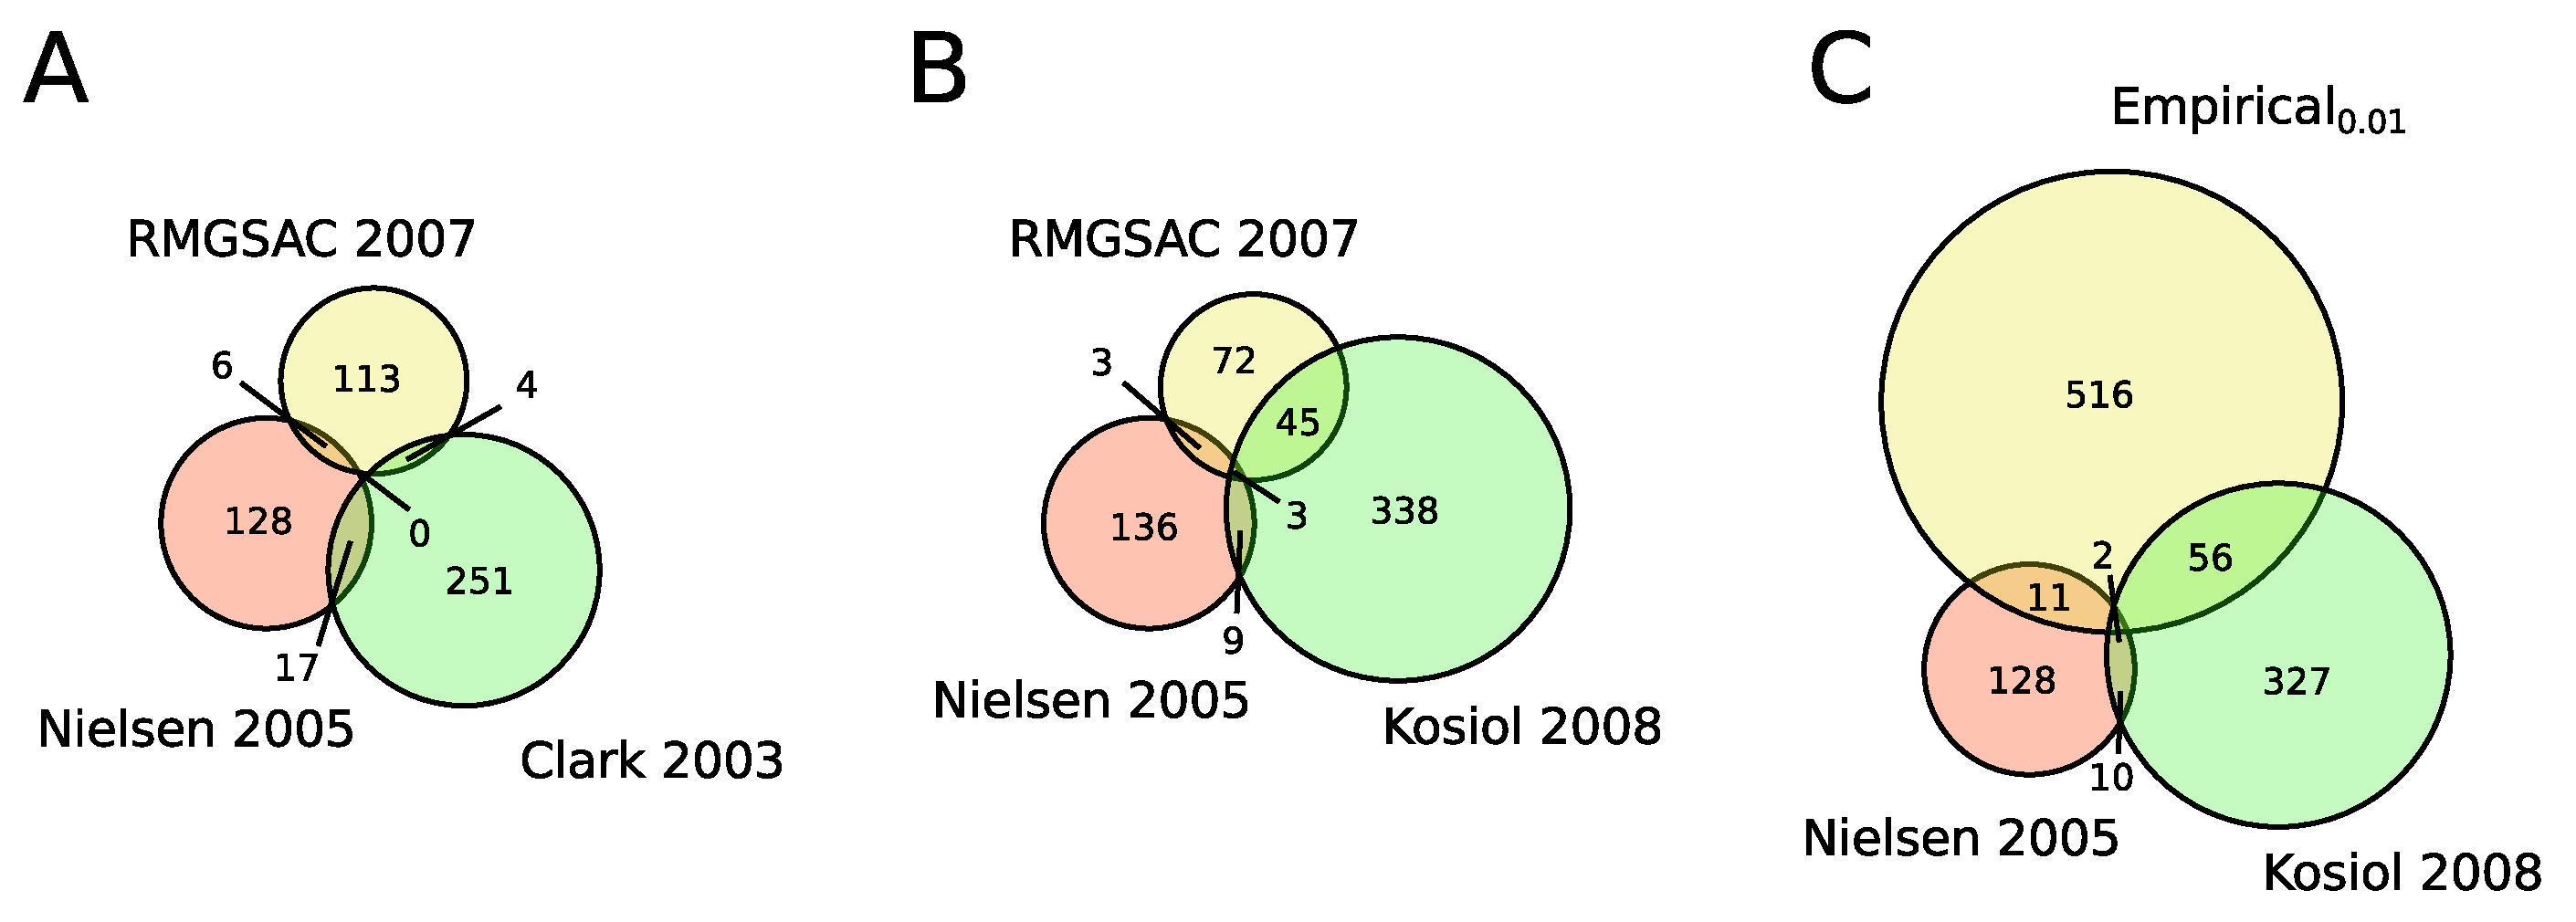
\includegraphics[scale=0.3]{Figs/pub_psg_venn.pdf}
\caption{Venn diagrams of \acp{psg} identified in different
  studies. (A) \acp{psg} identified in primates by Clark et
  al. \citeyearpar{Clark2003}, Nielsen et
  al. \citeyearpar{Nielsen2005} and the Rhesus Macaque Genome
  Sequencing and Analysis Consortium \citeyearpar{Macaque2007}. (B)
  \acp{psg} identified in primates and mammals by Nielsen et
  al. \citeyearpar{Nielsen2005}, the Rhesus Macaque Genome Sequencing
  and Anaalysis Consortium \citeyearpar{Macaque2007} and Kosiol et
  al. \citeyearpar{Kosiol2008}. (C) \acp{psg} identified in primates
  and mammals by Nielsen et al. \citeyearpar{Nielsen2005}, Kosiol et
  al. \citeyearpar{Kosiol2008} and this study using the Mammals
  species group, conservative filter, and the \psgeone method.}
\label{fig_pub_psg_venn}
\end{figure}

Figure \ref{fig_pub_psg_venn} shows the overlap between \acp{psg}
identified in this and previously-published studies. Note that the
total numbers of \acp{psg} are smaller than those noted in the
previous paragraph, as genes which were absent from the
conservatively-filtered dataset were removed. (Results from a
comparison using the relaxed filter were qualitatively similar to
those in Figure \ref{fig_pub_psg_venn}.) Overall, the lack of overlap
in identified \acp{psg} was striking: Figure \ref{fig_pub_psg_venn}A
shows the overlap between the three studies in primates, with zero
genes shared by all 3 studies and from 4 to 17 genes shared between
any pair. Although each analyses identified similar numbers of
\acp{psg}, very few of the actual genes identified were in
common. This result did not appear to be an artifact of genes lost
during the mapping process, as Nielsen et al. also noted that only 1
of their top 50 genes was also identified by Clark et
al. \citeyearpar{2003} as evolving under positive selection. Figure
\ref{fig_pub_psg_venn}B shows slightly more overlap between the two
most recent studies, with 45 \acp{psg} shared between Kosiol et
al. and the Rhesus genome analysis. The comparison between \acp{psg}
from Nielsen et al., Kosiol et al., and the set of \psgeone \acp{psg}
from the Mammals species group shown in Figure \ref{fig_pub_psg_venn}C
revealed a similar number of overlapping genes, despite the larger
overall number of \acp{psg} identified in the current study.

The comparison of overlapping \acp{psg} was somewhat limited, as it
required the use of a cutoff threshold to identify each set of
\acp{psg} and did not easily allow for a comparison between the
different methods. For example, although Figure
\ref{fig_pub_psg_venn}C showed a greater number of overlapping genes
between Kosiol et al. and the current study than between Nielsen et
al. and the current study (154 vs. 31), it was unclear whether this
was due to the greater overall number of \acp{psg} identified by
Kosiol et al., or to a greater tendency for this study and Kosiol et
al. to identify common \acp{psg}. By eye, it seemed as if both Kosiol
et al. and Nielsen et al. shared a similar proportion of \acp{psg}
with the current study.

As an alternative approach to comparing between the current results
and previous studies, I constructed a series of \ac{roc} curves for
each published study. For each study, the set of \acp{psg} was used as
the binary classifier (or ``truth'' value), and a set of 4 gene-wide
$p$-values or \dnds estimates from the current study were evaluated as
test statistics. Curves were constructed by sorting the list of
matched genes by each test statistic and counting the cumulative
number of \acp{psg} identified as the test statistic increased in
value. To test whether the choice of species group affected the
proportion of shared \acp{psg}, I included gene-wide \dnds estimates
for Primates and Mammals (where the test statistic was the negative
\dnds value, so the genes with highest \dnds were sorted first), and
to test whether the method used to combine \sw estimates within genes
had an effect, I included \psgeone and \psghoch $p$-values as test
statistics.

\begin{figure}
\centering
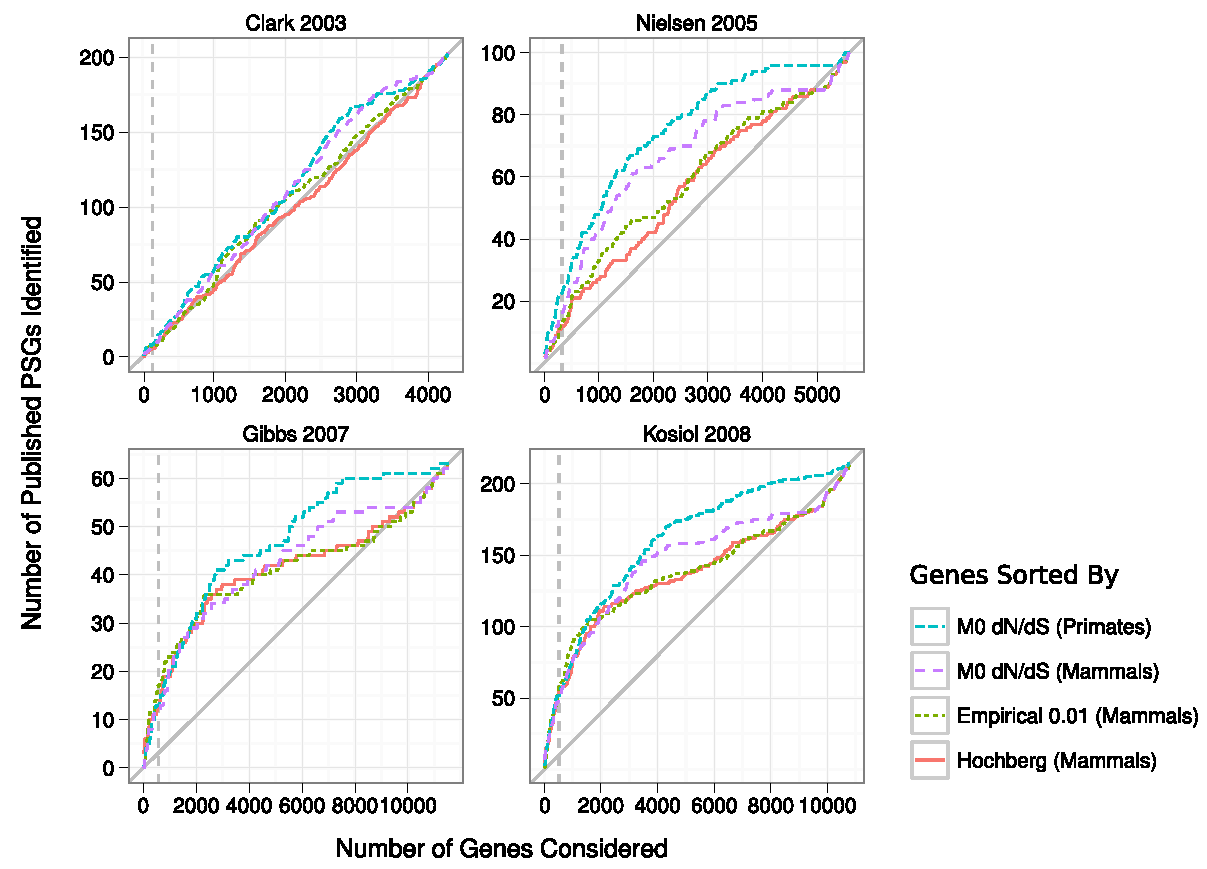
\includegraphics[scale=0.78]{Figs/psg_rocs.pdf}
\caption{\ac{roc} curves for using \dnds estimates and different
  \ac{psg} identification methods to identify \acp{psg} in
  previously-published studies. Within each panel, the x-axis
  represents all genes successfully matched between the published
  study and the current analysis and the y-axis represents the number
  of \acp{psg} within the matching genes. Each curve traces the
  cumulative number of \acp{psg} identified in the published study
  when the top $N$ genes, according to the test statistic, were
  considered. A dashed vertical line is drawn on each panel at the
  x-axis value corresponding to the number of \psgeone \acp{psg} in
  the Mammals species group.}
\label{fig_psg_rocs}
\end{figure}

Figure \ref{fig_psg_rocs} shows the \ac{roc} curves comparing the
current dataset to each of the four previously published studies. The
vertical dashed lines correspond to the FDR$<0.1$ threshold of the
\psgeone $p$-values in Mammals, making the intersection of the
\psgeone \ac{roc} curve at the vertical lines equivalent to the
numbers of overlapping \acp{psg} seen in Figure
\ref{fig_pub_psg_venn}C for the Nielsen et
al. \citeyearpar{Nielsen2005} and Kosiol et
al. \citeyearpar{Kosiol2008} sets of \acp{psg}.

The Clark et al. \citeyearpar{Clark2003} curves hardly strayed from
the diagonal line, showing little ability beyond random chance to
identify \acp{psg} from that study. This was not necessarily
unexpected, as that study tested for positive selection only along the
very short human and chimpanzee branches of the primate tree, while
even the Primates species group from the current study contained
sequences from species as distant as tarsier, covering much more
branch length and a much more diverse set of primate species. The
Nielsen et al. \citeyearpar{Nielsen2005} study showed a noticeably
stronger enrichment for \acp{psg} in genes with low $p$-values or high
\dnds values in the current study, with each \ac{roc} curve rising
well above the diagonal, and the Primates \dnds curve showing the
greatest performance. The difference between the curves for Nielsen et
al. and Clark et al. was interesting, as both studies used the same
set of sequences and alignments. Presumably the analytical method used
by Nielsen et al. was more similar to the current study in its
sensitivity to patterns of positive selection than that used by Clark
and colleagues. Within the Nielsen et al. panel, the difference
between the two curves based on overall \dnds ratios and the two
curves based on $p$-values from \sw estimates was noticeable, with the
\dnds curves showing greater performance throughout the range of
cutoff values. This may be explained by the small amount of branch
length included in that study providing only enough power to detect
\acp{psg} with high overall \dnds values as opposed to genes with
smaller proportions of positively-selected sites.

The \ac{roc} curves for the two more recent studies showed noticeably
greater, and roughly equivalent, performance. In both cases, all 4
curves showed nearly identical performance in the high-specificity
region of the graph, identifying roughly 25\% of the total number of
\acp{psg} were identified by all curves before the vertical dashed
line was reached. At the same significance threshold, roughly 20\% and
2\% of \acp{psg} were identified in the Nielsen et al. and Clark et
al. graphs, respectively. The curves based on \dnds values showed
better performance than the \sw methods at the higher end of the
curve; this was somewhat expected, as the \psgeone and \psghoch
methods both required reasonably strong \sw evidence for positive
selection to successfully distinguish between \acp{psg} and
non-\acp{psg}. The observation that the \sw methods were less able
than \dnds values to identify \acp{psg} from the Rhesus consortium and
Kosiol et al. in the low-specificity range was consistent with a
slight lack of power to detect weak distributed positive selection
resulting from the use of \sw estimates to identify \acp{psg}.

\section{Gene families with many \acp{psg}}

Table \ref{table_go} contained a relatively large number of \acp{psg}
from the same gene family (e.g., solute carrier family genes
\gene{SLC26A8}, \gene{SLC16A7}, \gene{SLC4A1}, \gene{SLC13A2},
\gene{SLC9A10}; collagen genes \gene{COL1A2}, \gene{COL4A3},
\gene{COL16A1}; and toll-like receptor genes \gene{TLR1} and
\gene{TLR4}). The clustering of \acp{psg} within large gene families
was not unexpected, as different members of a gene family may be more
likely to have similar cellular functions; thus, a family of
immune-related genes such as the TLR genes would be expected to be
enriched for \acp{psg}. The prevalence of positively-selected gene
family members was concerning, however, as many gene families arise
through segmental duplications \citep{Ohno1970}, and duplicate genes
residing nearby on a chromosome are likely targets of ectopic gene
conversion events \citep{Ezawa2006,Benovoy2009}. Gene conversion is a
non-reciprocal recombination process which is initiated by a
double-stranded break in the DNA helix that is subsequently repaired
through strand invasion by a homologous sequence; ectopic gene
conversion events are defined as those that occur between homologous
sequences not at the same genetic locus \citep{Benovoy2009}. The
problem with gene conversion in comparative studies is that it breaks
the assumption that the relationships of a set of genes can be well
described by one bifurcating phylogenetic tree. Thus, when sequences
with gene conversion are analyzed using the species tree, an incorrect
sequence of substitution events is required to explain the observed
sequences with respect to the phylogenetic tree, potentially leading
to excessive estimates of substitution rates. In the case of detecting
positive selection, gene conversion among paralogs has been observed
to result in moderately elevated rates of false positives
\citep{Casola2009}.

\begin{table}
\centering \footnotesize
\begin{tabular}{lrrrrrl}

\toprule

Gene Family & Genes & NPPs & PSGs &
\multicolumn{2}{l}{NPP--PSGs} & Top 4 NPP--PSGs \\

\midrule
\multicolumn{4}{l}{Ensembl Families with $>4$ \acp{psg}} & & & \\
\midrule

\input{Tables/psg_fams_ensf.txt}

\midrule
\multicolumn{4}{l}{Manually Curated Families} & & \multicolumn{2}{l}{FET $p$-value} \\
\midrule

\input{Tables/psg_fams_custom.txt}

\bottomrule
\end{tabular}
\caption{}
\label{table_psg_fams}
\end{table}

I assessed the potential impact of gene conversion on the current
dataset by identifying \acp{npp} and comparing those to the list of
\psgefive \acp{psg} from the relaxed \sw filter and the Mammals
species group. I defined \acp{npp} as pairs of genes which are members
of the same \ens gene family and which reside on the same chromosome
within 2 Mb of each other; in total, 1,150 genes from 361 \ens
families were identified as members of a \ac{npp}. The top section of
Table \ref{table_psg_fams} summarizes the coincidence of \acp{npp}
and \acp{psg} within Ensembl gene families containing at least 3
\acp{psg}, sorted by the number of genes which were both \acp{psg} and
part of a \ac{npp}. The list was topped by the collagen type IV
family, with all 6 family members showing evidence of positive
selection in mammals and residing within 2Mb of another family
member. Other families containing many \ac{npp}--\acp{psg} were the
CD1 family of transmembrane glycoproteins \citep{Joyce2001}, several
members of the complement immune system \citep{Nonaka2006}, a family
of guanylate-binding proteins located in a cluster on chromosome 1
\citep{Olszewski2006}, and two families containing granzyme peptidases
and serine peptidase inhibitors.

Every \ac{psg} from the aforementioned families was also a member of a
\ac{npp}, suggesting that gene conversion may have led to the false
detection of positive selection in these families. However, many of
the same families contained genes involved in core immune system
processes which have been consistently shown to harbor the highest
fraction of \acp{psg}. Thus, although these gene families exhibited a
striking coincidence of \acp{npp} and \acp{psg}, the impact of such
co-occurrence on the false detection of positive selection within any
one family was highly dependent on the function of genes within that
family and the associated prevalence of true \acp{psg}. Regardless of
this complication, it could be asserted that gene families from the
top section of Table \ref{table_psg_fams} represented those with the
highest likelihood of false positives resulting from gene
conversion. A more in-depth study of the evolution of each family
would be necessary to confidently assess whether individual families
or genes contained evidence of false positives resulting from gene
conversion events. Of particular interest were the families without
obvious involvement in well-known systems of genetic conflict and
positive selection, such as the collagen (e.g., \gene{COL4A6}),
carboxylesterase (e.g., \gene{CES5A}), solute carrier family (e.g.,
\gene{SLC22A25} and \gene{SLC17A3}), and matrix metallopeptidase
(e.g., \gene{MMP3}) families.

\begin{table}
\centering \footnotesize
\begin{tabular}{llrllllr}

\toprule

\multicolumn{3}{c}{Human Gene} & \multicolumn{3}{c}{Evidence for Positive Selection} & & \\
\cmidrule(r){1-3} \cmidrule(r){4-6}
Name & Chr. & Loc. & Relaxed & Conservative & Lit. & \ac{npp} & \psgeone $p$-value \\

\midrule

\input{Tables/psg_col_mmp.txt}

\bottomrule
\end{tabular}
\caption{}
\label{table_psg_col_mmp}
\end{table}

The presence of metallopeptidase and collagen gene families in Table
\ref{table_psg_fams} was especially intriguing, as members of the
metallopeptidase class of enzymes are responsible for breaking down
collagen fibers in the extracellular matrix with various specificities
\citep{Sluijter2006}. Table \ref{table_psg_col_mmp} summarizes the
collagen and metallopeptidase genes which showed evidence of positive
selection; the signal of positive selection was much stronger in the
type IV collagen genes than in the metallopeptidases, and all genes
with evidence for positive selection were members of a \ac{npp}. If
gene conversion among these \acp{npp} can be ruled out, then the
presence of positive selection within these gene families may be
suggestive of either an undescribed relationship between type IV
collagen fibers and the immune system ``arms race'', or a novel type
of genetic conflict underlying the presence of positive selection in
these related gene families.

Within larger gene groups and across the genome-wide dataset, Fisher's
exact test could be used to test the hypothesis of independence
between \acp{npp} and \acp{psg}, providing some quantitative evidence
for or against the hypothesis that \acp{npp} were involved in the
false positive detection of \acp{psg}. The bottom section of Table
\ref{table_psg_fams} shows the results of this test for four
manually-curated gene superfamilies and the entire set of 15,946 genes
from the relaxed dataset in the Mammals species group. While there was
little evidence for non-independence between these two factors for the
group of 8 toll-like receptors, \ac{fet} yielded low $p$-values for
the 30 collagen genes and 42 ADAM family genes, a significant
$p$-value for the 338 solute carrier family genes, and a highly
significant result for non-independence across the entire genome. This
result provided strong evidence that the distribution of \acp{npp} and
\acp{psg} was highly non-uniform; evaluated in the context of previous
results showing that gene conversion can lead to false positives in
detecting positive selection, this suggested that the evidence for
positive selection within \acp{npp}--\acp{psg}, some of which have
been identified in previous studies (e.g., \gene{COL4A6} and
\gene{COL4A3} from Table \ref{table_psg_col_mmp} which were identified
by Kosiol et al. \citeyearpar{2008}) should be treated with caution.

\section{Positive and purifying selection within protein-coding domains}

Using the same methodology developed for genes, \sw estimates could be
grouped by other entities of interest to assess levels of purifying
and positive selection within those groups. An interesting application
of this approach was the use of \sw data to identify protein-coding
domains showing the strongest genome-wide evidence for positive
selection. Although the gene-wise results could be used to identify
protein domains often shared by \acp{psg}, the direct assessment of
levels of purifying and positive selection within domains had the
potential to more sensitively and accurately identify positive
selection...

\section{Conclusions}

